\section{Class diagram}
\subsection{Description}
\begin{flushleft}
Dans cette section, nous découvrirons les différentes classes liées à l'implémentation des différentes fonctionnalités.
\end{flushleft}

\begin{flushleft}
Tout d'abord, le schéma ci-dessous ne reprend que la classe de l'extension (étant donné que le schéma est suffisament grand et est déjà disponible plus haut). La classe "Facture" est reliée à la classe ClientApi puisque que cette extension n'est disponible que pour les clients.
\end{flushleft}

\subsection{Les variables}
\begin{flushleft}
Dans la classe Facture, plusieurs arguments sont répertoriés.
\end{flushleft}

\begin{enumerate}[-]

\item \textbf{La variable "paiement_status" permet de voir le statut de paiement de la facture via un boolean (payed=true).}

\item \textbf{La variable "ideal_accompt" affiche l'accompte calculé automatiquement par l'application via un double.}

\item \textbf{La variable "paiement_method" affiche la méthode de paiement via un boolean (manual=true).}

\item \textbf{La variable "paiement_informations" affiche, sous forme d'une ArrayList, les informations de paiement.}

\item \textbf{La variable "factures_history", de la même manière que la variable précédente, affiche un historique des factures du client.}

\item \textbf{La variable "proposal" contient, sous forme d'un double, la proposition du client lorsqu'il modifie la proposition faite par l'application.}

\end{enumerate}

\subsection{Les méthodes}
\begin{flushleft}
Plusieurs méthodes de cette classe permettent l'implémentation des factures.
\end{flushleft}

\begin{enumerate}[-]

\item \textbf{La méthode "checkStatus" permet de vérifier le statut de paiement d'une facture.}

\item \textbf{La méthode "calculateAmount" est la méthode par laquelle l'application va calculer le montant idéal.}

\item \textbf{La méthode "checkProposal" permet à l'application de vérifier les conditions de la proposition du client.}

\item \textbf{La méthode "changePaiementMethod" permet au client de modifier son mode de paiement.}

\item \textbf{La méthode "changePaiementInformations" modifie les informations bancaires du client à sa volonté.}

\item \texbf{Dans le cas où le paiement manuel est choisi, la méthode "generateQRCode" est appelée afin de générer un QR Code correpsondant au paiement.}

\item \textbf{La méthode "sendNotification" envoie une notifications (via une application externe) lorsque qu'un facture est disponible.}

\item \textbf{La méthode "seeHistory" permet au client de voir la liste de ses factures. Chaque facture sera ajoutée dans la liste des factures.}

\item \textbf{La méthode "checkIsPayed" est une méthode liée au paiement de vérifier si le paiement est validé ou pas.}

\item \textbf{La class est munie d'un constructeur "Facture" créant l'objet Facture pouvant être ajouté dans l'ArrayList.}

\end{enumerate}

\begin{figure}[h]
\subsection{Schéma}
\centering
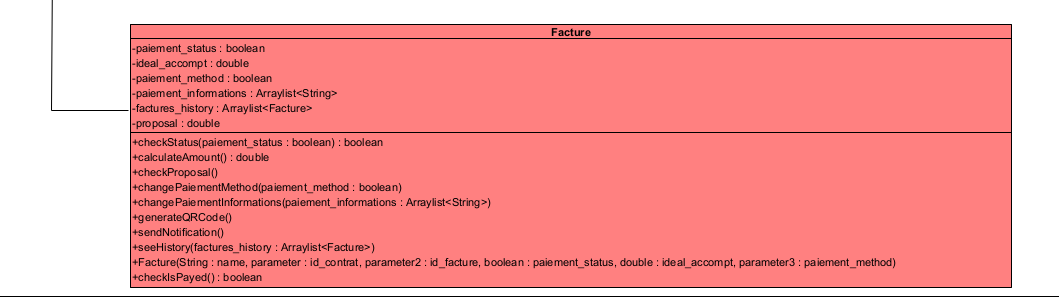
\includegraphics[width = 1]{extension-maxime/class/img/class-extension.png}
\end{figure}


